\chapter{Dynamics}\label{chap:dynamics}
This chapter contains an analysis of the dynamics of the pan/tilt system which will result in a mathematical model. Calculations made throughout this chapter resides in appendix \ref{app:dynamics_calc}. Identifying and understanding the relevant dynamics of a system is important as this will lead to an as accurate theoretical model as needed for the application. Ideally a perfect model would somewhat be preferred, but it would be a very difficult and tedious task to derive a perfect model and completely unnecessary. The reason for that is some of the dynamics are insignificant to the behaviour of the system, others might have a little impact on the behaviour and can be omitted due to more dominating dynamics. The response of electrical circuits are often much quicker than the response of a mechanical system. This response delay is encoded into the poles of a system, making the poles of the system very interesting to analyse. The poles of the system tell if it is stable, and if any dynamics in the system possibly can be omitted due to its relatively fast response compared to the rest of the system which acts slower.

A system can always be constructed of first order systems and second order systems in a cascade. These two types of systems define a time constant. For first order systems the time constant can be derived from the zeroth order term and in second order systems it can be derived from the first order term. From a physical point of view the time constant defines the point in time where the system reaches $1 - \sfrac{1}{e} \approx 63.2\%$ of its final energy state, below in figure \ref{fig:energy_systems} is illustrated a step response on a first and a second order system.
\begin{figure}[htb]
	\centering
	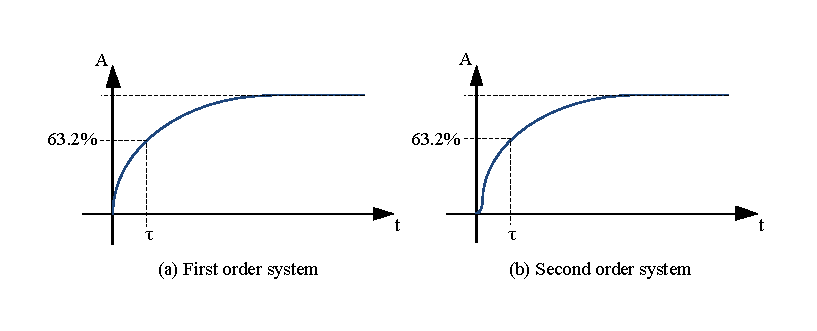
\includegraphics[scale=1,trim=0 0 0 0]{graphics/energy_systems.pdf} %trim=l b r t (can cut off from every side)
	\caption{(a) Illustrates the step response of a first order system. (b) Illustrates a step response of a second order system. Both will raise in time and reach some asymptotic value provided that the systems are stable, $\tau$ denotes the time constant.}
	\label{fig:energy_systems}			% figure labels are of the form \label{fig:*}
\end{figure}
In figure \ref{fig:energy_systems}(b), notice the transient which seems more inert compared to (a). This is due to some mass in the system if the second order differential equation which represents the system is a mechanical equation. The transient response of a system is encoded into the poles of the system, which is defined by the time constant the following way:
\begin{equation}
	\tau = \frac{1}{\zeta\omega_{n}}\label{eq:time_constant}
\end{equation}
where $\zeta$ is the dampening ratio and $\omega_{n}$ is the undampened natural frequency, this relates to the poles as seen in figure \ref{fig:s_plane}.
\begin{figure}[htb]
	\centering
	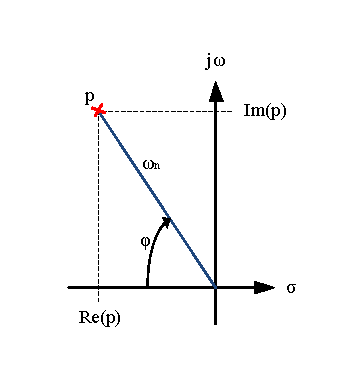
\includegraphics[scale=1,trim=0 0 0 0]{graphics/splane.pdf} %trim=l b r t (can cut off from every side)
	\caption{This figure illustrates a pole in the s-plane and the relation between poles and time constants.}
	\label{fig:s_plane}			% figure labels are of the form \label{fig:*}
\end{figure}
In figure \ref{fig:s_plane} the real part of the pole is given by $Re(p) = - \zeta\omega_{n} = - \omega_{n} \cos(\varphi)$ and the imaginary part is given by $Im(p) = j\omega_{n}\sqrt{1 - \zeta^{2}} = j\omega_{n}\sin(\varphi)$. Considering equation \ref{eq:time_constant} and figure \ref{fig:s_plane} it can be seen that the real part of a pole directly relates to the time constant. Systems with one pole can therefore have their time constant calculated from the reciprocal of the real part of the pole. Systems consisting of more than one pole can have their time constant calculated from the super positioning the reciprocal of the real part of the poles. Equation \ref{eq:time_constant} show an example.
\begin{equation}
	\tau = \frac{1}{Re(p_{1})} + \frac{1}{Re(p_{2})} + \frac{1}{Re(p_{3})} + ... + \frac{1}{Re(p_{N})}\label{eq:time_constant}
\end{equation}
As the time constant is defined as the reciprocal of the real part of the pole, then poles far away from the imaginary axis will not add that much to the total time constant as poles located near the imaginary axis. Therefore the following can be concluded, much \textit{faster} poles in a system containing \textit{slower} poles can be omitted from the model of the system.

\section{Overview of pan/tilt}
The following will give an overview of the physical aspects of the pan/tilt system and also define the mathematics which is tied to the system. The pan/tilt is assembled from two motors, a set of gears connected to each motor. Each motor can rotate a mass individually by transferring torque from the motors, through the gears, to the masses which are connected to the gears. A model of the motors are needed, along with a model of the reflected inertia through the gears, and other dynamics might be relevant to, but are discussed later in this section.

\subsection{Motor}
The motor converts electrical energy to mechanical energy as a voltage is supplied to the motor. This voltage make the motor turn and this turning motion deliver torque though some gears to a mass which then spins up to some maximum speed. A simplification of a DC motors circuit can be seen in figure \ref{fig:motor_circuit}, from this a mathematical model of the motor can be derived.
\begin{figure}[htb]
	\centering
	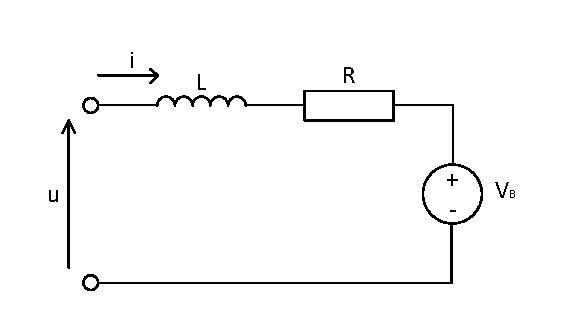
\includegraphics[scale=1,trim=0 0 0 0]{graphics/motor_circuit.pdf} %trim=l b r t (can cut off from every side)
	\caption{Simplification of circuit for a DC motor. Voltage supplied is denoted by $u$, $i$ is the current through the motor, $L$ is inductance, $R$ is resistance and $V_B$ is the the voltage generated from the coil rotating in a magnetic field.}
	\label{fig:motor_circuit}			% figure labels are of the form \label{fig:*}
\end{figure}
Following can be derived from the circuit seen in figure \ref{fig:motor_circuit}.
\begin{align}
	u &= L\frac{di}{dt} +  Ri + V_B \Longleftrightarrow\\
	u &= L\frac{di}{dt} +  Ri + K_B\omega\label{eq:motor_model}
\end{align}
where $u$ is the voltage input, $i$ is the current, $\frac{di}{dt}$ is the time derivative of the current, $L$ is the inductance, $R$ is the resistance and $V_B$ is the voltage generated in the in coil of the motor as it spins in a magnetic field. $V_B$ can be expressed by $K_B$ which is the \textit{back-emf}\footnote{EMF is an abbreviation for electromotive force, which is the voltage generated from a coil rotating in a magnetic field.}-constant, times $\omega$, which is the angular velocity of the motor. As the motors need to move a mass an expression for torque is more interesting compared to the expression derived in \ref{eq:motor_model}. The electrical torque can be expressed in the following way:
\begin{equation}
	\tau = K_Ti\label{eq:electrical_torque}
\end{equation}
where $K_T$ is the torque constant.	The mechanical torque can be expressed in the following way:
\begin{equation}
	\tau = J_L\frac{d\omega}{dt}\label{eq:mechanical_torque}
\end{equation}
where $J_L$ is the inertial load on the motor, $\frac{d\omega}{dt}$ is the time derivative of the angular velocity of the motor. Equation \ref{eq:electrical_torque} and \ref{eq:mechanical_torque} equals each other if it is assumed that the energy is conserved in the transfer from electrical to mechanical torque. The following expression is obtained then obtained from equation \ref{eq:electrical_torque} and \ref{eq:mechanical_torque}:
\begin{align}
	K_Ti &= J_L\frac{d\omega}{dt} \Leftrightarrow\\
	i &= \frac{J_L}{K_T} \frac{d\omega}{dt}\label{eq:electrical_mechanical_torque}
\end{align}
To derive $\frac{di}{dt}$ the time derivative is taken of \ref{eq:electrical_mechanical_torque} which leads to:
\begin{equation}
	\frac{di}{dt} = \frac{J_L}{K_T} \frac{d^{2}\omega}{dt^{2}}\label{eq:electrical_mechanical_torque_derivative}
\end{equation}
Now \ref{eq:electrical_mechanical_torque} and \ref{eq:electrical_mechanical_torque_derivative} can be substituted into \ref{eq:motor_model} in which the following is obtained:
\begin{equation}
	u = \frac{L J_L}{K_T} \frac{d^{2}\omega}{dt^{2}} + \frac{R J_L}{K_T} \frac{d\omega}{dt} + K_B \omega\label{eq:model_model}
\end{equation}

Stiction, coulomb and viscous friction are omitted as it is assumed that the inertia from the internal friction of the motor is a lot less than the inertia from the mass, so this concludes the model of the motor.

\subsection{Gears}
The gears between the mass to be rotated and the motor of the system reflect the actual inertia of the mass onto the motor. Calculations for the reflected inertia is kept in appendix \ref{app:dynamics_calc}.
  
\subsection{Torque-induced precession}
When a body rotates around an axis the phenomenon of precession occurs. The torque-induced precession occurs when a body accelerates around an axis a torque is induced perpendicular to the axis of rotation. In figure \ref{fig:precession} a sketch of this situation is shown.
\begin{figure}[htb]
	\centering
	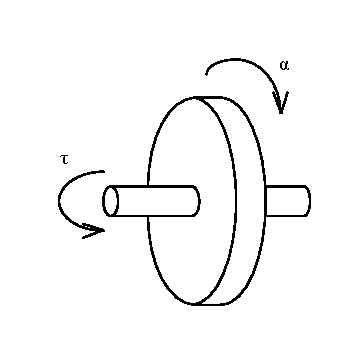
\includegraphics[scale=1,trim=0 0 0 0]{graphics/precession.pdf} %trim=l b r t (can cut off from every side)
	\caption{Shows the concept of of the torque-induced precession.}
	\label{fig:precession}			% figure labels are of the form \label{fig:*}
\end{figure}
This torque is given by:
\begin{equation}
	\tau = I\alpha\label{eq:induced_torque}
\end{equation}
where $\tau$ is the torque, I is the inertia of the body rotating and $\alpha$ is the angle acceleration the body is affect by. An example is that if the tilt part of the system is accelerating up to some velocity, a torque will be applied to the pan part of the system, this torque is acting perpendicular to the rotation causing the pan to rotate as long as the motor for the tilt part is accelerating. To investigate the impact of the torque-induced precession, equation \ref{eq:motor_model} and \ref{eq:induced_torque} have to be related to each other. As equation \ref{eq:induced_torque} is expressed as torque, equation \ref{eq:motor_model} is rewritten with respect to torque. equation \ref{eq:mechanical_torque}.
\begin{equation}
	J_L \frac{d\omega}{dt} = \frac{K_T}{R} u - \frac{L J_L}{R} \frac{d^{2}\omega}{dt^{2}} - \frac{K_B K_T}{R} \omega\label{eq:torque_motor_model}
\end{equation}
Then equation \ref{eq:induced_torque} is subtracted from the total torque \ref{eq:torque_motor_model} as follows:
\begin{equation}
	J_L \frac{d\omega_{1}}{dt} = \frac{K_T}{R} u - \frac{L J_L}{R} \frac{d^{2}\omega_{1}}{dt^{2}} - \frac{K_B K_T}{R} \omega_{1} - I \frac{d\omega_{2}}{dt}\label{eq:coupled_torque_motor_model}
\end{equation}
where $\omega_1$ is the velocity of the pan and $\omega_2$ is the velocity of the tilt. 

\section{Finding parameters}
The following will contain a brief discussion on how the parameters were found. To obtain the parameters for the model some measurements where made on tilt part of the system. These measurements and the MATLAB script which was used for analysing the data is located on the CD. The measurements that where produced is expressed in encoder $[ticks]$ against time $[ms]$. All the previous equations are dependent of the velocity of the system, so the measurements have to be differentiated with respect to time, this is done by a numerical method called the secant method\footnote{NR ref}, the differentiated result is plotted and shown in figure \ref{fig:measured_step_tilt}.
\begin{figure}[htb]
	\centering
	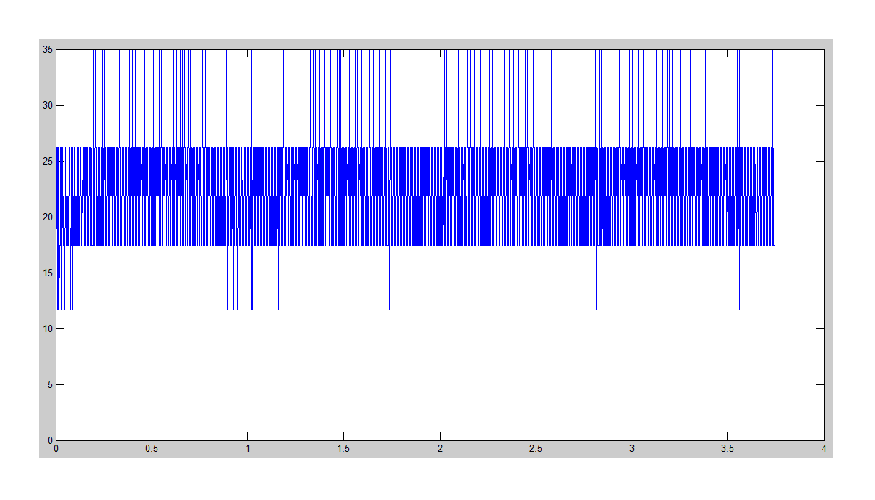
\includegraphics[width=\textwidth]{graphics/measured_step_tilt.pdf} %trim=l b r t (can cut off from every side)
	\caption{This graph show the actual velocity of the tilt part of the system. The horizontal axis show time in seconds. The vertical axis show angular velocity in radians per second.}
	\label{fig:measured_step_tilt}			% figure labels are of the form \label{fig:*}
\end{figure}
If a mean is calculated from the steady-state part of the graph $22.57 \sfrac{rad}{s}$ is obtained, and compared to the data sheet of the motor which says the rated speed is $22.62 \sfrac{rad}{s}$, the data from the graph represented in figure \ref{fig:measured_step_tilt} is assumed to be correct.

Next a set of equations are formed from equation \ref{eq:model_model}, the input is set to zero and rewritten as follows:
\begin{equation}
	\frac{d^{2}\omega}{dt^{2}} = - \frac{R}{L} \frac{d\omega}{dt} - \frac{K_B K_T}{L J_L} \omega
\end{equation}
where $\frac{d^{2}\omega}{dt^{2}}$, $\frac{d\omega}{dt}$, and $\omega$ is known, from numerical analysis, so the constants $\frac{R}{L}$ and $\frac{K_B K_T}{L J_L}$ can be found. $R$ and $J_L$ are also known and $K_B = K_T$. MATLAB have been used for calculating the set of equations $\textbf{Ax} = \textbf{b}$, so that the rest of the unknowns can be found. The MATLAB script located on the CD contains further details about how the set of equations where formed.

\subsection{Verification}
Previous experiments and calculations have shown that $R = 5.124\Omega$, $L = 38.4mH$ and $K_B = K_T = 35.1 \sfrac{mV}{\dfrac{rad}{s}}$. Through the MATLAB script included on the CD, $\frac{R}{L}$ and $\frac{K_B K_T}{L J_L}$ is found to be the following:
\begin{equation}
	\frac{R}{L} = 791.7 \Rightarrow L = \frac{5.124}{791.7} \approx 6.471mH
\end{equation}
\begin{equation}
	\frac{K_B K_T}{L J_L} = 25.63\label{eq:constants}
\end{equation}
According to equation \ref{app:eq_reflected_pan_inertia}, $J_L = 0.970 \cdot 10^{-3} kg \cdot m^{2}$ which is the reflected inertia of the tilt part through the gears, $L = 6.471mH$, and $K_B = K_T$. Now $K_B$ and $K_T$ can be calculated the following way:
\begin{equation}
	K_B = K_T = \sqrt{25.63 \cdot L \cdot J_L} \Rightarrow K_B = K_T = \sqrt{25.63 \cdot L \cdot J_L} \approx 401.1 \frac{mV}{\sfrac{rad}{s}}
\end{equation}
By looking at a pole-zero plot of the system and the open-loop response of the system, it can be decided which set of parameters that can be used for setting up the model. To set up the model a state-space representation is made of the system as follows below. The coupled system is set up with respect to equation \ref{eq:coupled_torque_motor_model}:
\[
 \dot{\textbf{x}} =
 \begin{bmatrix}
   0 & 1 & 0 & 0\\
   - \frac{K_B K_T}{L J_{Pan}} & - \frac{R}{L} & 0 & - \frac{I_{Tilt}}{J_{Tilt}}\\
   0 & 0 & 0 & 1\\
   0 & - \frac{I_{Pan}}{J_{Pan}} & - \frac{K_B K_T}{L J_{Tilt}} & - \frac{R}{L}
 \end{bmatrix}
 \textbf{x} +
 \begin{bmatrix}
   0 & 0\\
   \frac{K_T}{L J_{Pan}} & 0\\
   0 & 0\\
   0 & \frac{K_T}{L J_{Tilt}}
 \end{bmatrix}
 \textbf{u}
\]
where the state vector $\textbf{x}$ is as follows:
\[
 \textbf{x} =
 \begin{bmatrix}
   \omega_{Pan}\\
   \dot{\omega_{Pan}}\\
   \omega_{Tilt}\\
   \dot{\omega_{Tilt}}\\
 \end{bmatrix}
\]
The two set of parameters are inserted into the model, parameters from previous experiments are inserted first which leads to: $R = 5.124\Omega$, $L = 38.4mH$, and $K_B = K_T = 35.1 \sfrac{mV}{\dfrac{rad}{s}}$. $J_{Pan}$, $J_{Tilt}$, $I_{Pan}$, and $I_{Tilt}$ can be found in appendix \ref{app:dynamics_calc}.
\begin{equation}
 \dot{\textbf{x}} =
 \begin{bmatrix}
   0 & 1 & 0 & 0\\
   - 16.9754 & - 133.4375 & 0 & - 100\\
   0 & 0 & 0 & 1\\
   0 & - 100 & - 33.0759 & - 133.4375
 \end{bmatrix}
 \textbf{x} +
 \begin{bmatrix}
   0 & 0\\
   483.6310 & 0\\
   0 & 0\\
   0 & 942.3325
 \end{bmatrix}
 \textbf{u}\label{eq:crap_ss_model}
\end{equation}
The eigenvalues of the A matrix is calculated in MATLAB to be:
\begin{equation}
 \lambda =
 \begin{bmatrix}
   - 233.3303\\
   - 32.6712\\
   - 0.7790\\
   - 0.0946
 \end{bmatrix}\label{eq:crap_eig_val}
\end{equation}
Looking at the values in \ref{eq:crap_eig_val} show that the last value of the vector is really close to zero which mean that the system is close to marginal stable. The open-loop response of the system is plotted in figure \ref{fig:crap_step}.
\begin{figure}[htb]
	\centering
	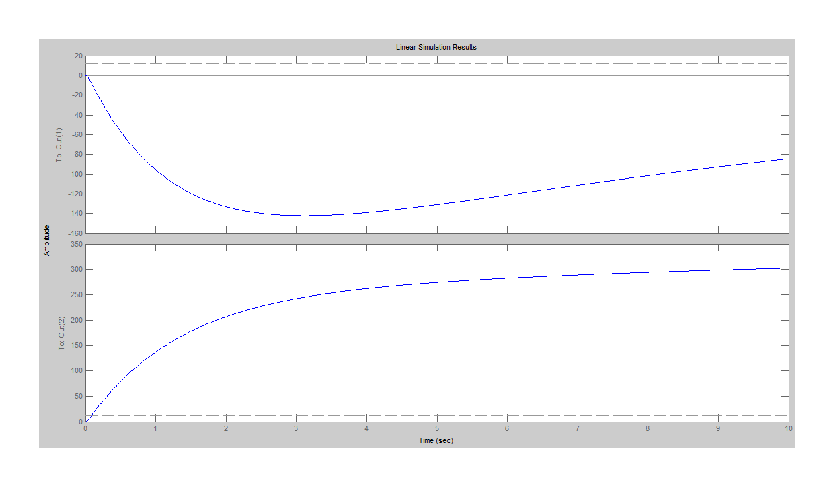
\includegraphics[width=\textwidth,trim=0 0 0 0]{graphics/CrapSim.pdf} %trim=l b r t (can cut off from every side)
	\caption{This figure illustrates the open-loop step response of the system in equation \ref{eq:crap_ss_model}.}
	\label{fig:crap_step}			% figure labels are of the form \label{fig:*}
\end{figure}
The step response in figure \ref{fig:crap_step} show some instability as a steady state response is never achieved.  compared to the figure, so the parameters from earlier experiments can not be used. The top graph of figure \ref{fig:crap_step} represent the pan part and the lower graph represent the tilt part. Same procedure is made with the calculated set of parameters, the parameters are $R = 5.124\Omega$, $L = 6.471mH$, and $K_B = K_T = 401.1 \frac{mV}{\sfrac{rad}{s}}$. $J_{Pan}$, $J_{Tilt}$, $I_{Pan}$, and $I_{Tilt}$ can be found in appendix \ref{app:dynamics_calc}.
These parameters leads to the following model:
\begin{equation}
 \dot{\textbf{x}} =
 \begin{bmatrix}
   0 & 1 & 0 & 0\\
   - 13153.8453 & - 791.7958 & 0 & - 100\\
   0 & 0 & 0 & 1\\
   0 & - 100 & - 25629.6574 & - 791.7958
 \end{bmatrix}
 \textbf{x} +
 \begin{bmatrix}
   0 & 0\\
   32794.2344 & 0\\
   0 & 0\\
   0 & 63898.0443
 \end{bmatrix}
 \textbf{u}\label{eq:super_ss_model}
\end{equation}
The \textbf{A}-matrix in equation \ref{eq:super_ss_model} got the following eigenvalues:
\begin{equation}
 \lambda =
 \begin{bmatrix}
   - 869.7571\\
   - 662.0630\\
   - 16.6873\\
   - 35.0842
 \end{bmatrix}\label{eq:super_eig_val}
\end{equation}
Eigenvalues in equation \ref{eq:super_eig_val} indicate the model in equation \ref{eq:super_ss_model} is stable which is expectable as the system is driven by motors which has a limitation in speed. A plot of the coupled system is shown in figure \ref{fig:good_step}.
\begin{figure}[htb]
	\centering
	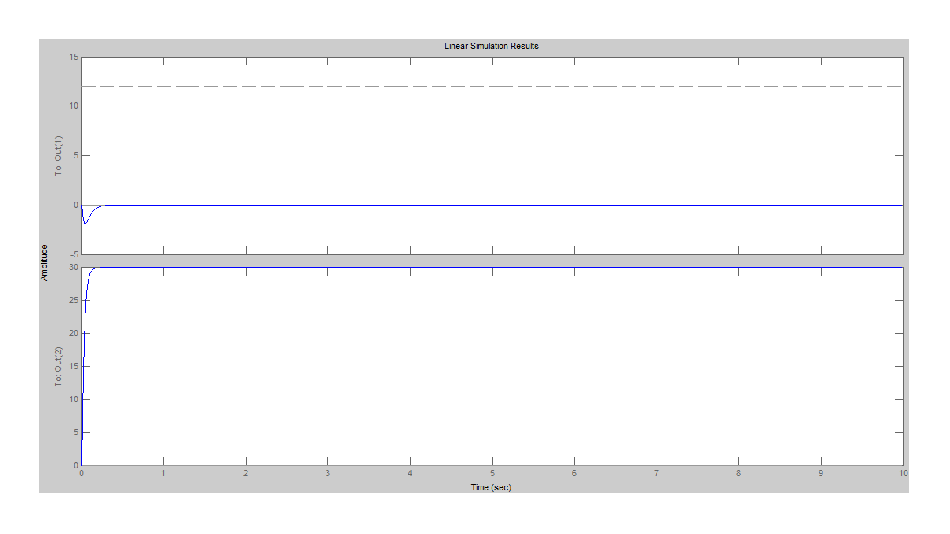
\includegraphics[width=\textwidth,trim=0 0 0 0]{graphics/GoodSim.pdf} %trim=l b r t (can cut off from every side)
	\caption{This figure illustrates the open-loop step response of the system in equation \ref{eq:super_ss_model}.}
	\label{fig:good_step}			% figure labels are of the form \label{fig:*}
\end{figure}
In figure \ref{fig:good_step} a simulation of the open-loop step response is represented, the top graph is the pan part and the lower graph is the tilt. The amplitude is representing angular velocity of the motors, the system have been excited with a $12V$ step on the motor which controls the tilt part, notice that the pan is affected of the tilt accelerating to about $30\sfrac{rad}{s}$ which is not far from $22.57\sfrac{rad}{s}$ which was measured and shown in figure \ref{fig:measured_step_tilt}. The offset can be explained by all the omitted dynamic such as friction in the system. This offset can be adjusted with an overall gain. The gain can be found the following way:
\begin{equation}
	Gain = \frac{Actual\ velocity}{Estimated\ velocity} = \frac{22.57\sfrac{rad}{s}}{30\sfrac{rad}{s}} = 0.7523\label{eq:gain_constant}
\end{equation}
The calculated gain can be put into the \textbf{C}-matrix of the model in the following way:
\begin{equation}
 \textbf{y} =
 \begin{bmatrix}
   0.7523 & 0 & 0 & 0\\
   0 & 0 & 0.7523 & 0
 \end{bmatrix}
 \textbf{x} +
 \begin{bmatrix}
   0 & 0\\
   0 & 0
 \end{bmatrix}
 \textbf{u}\label{eq:output_ss_model}
\end{equation}
The state space model can now be formed from equation \ref{eq:super_ss_model} and \ref{eq:output_ss_model}. The output have been plotted in the graph below, the blue line is the open-loop response of the state-space model with a gain of $1$ and the green is the response of the model with the calculated gain from equation \ref{eq:gain_constant}.
\begin{figure}[htb]
	\centering
	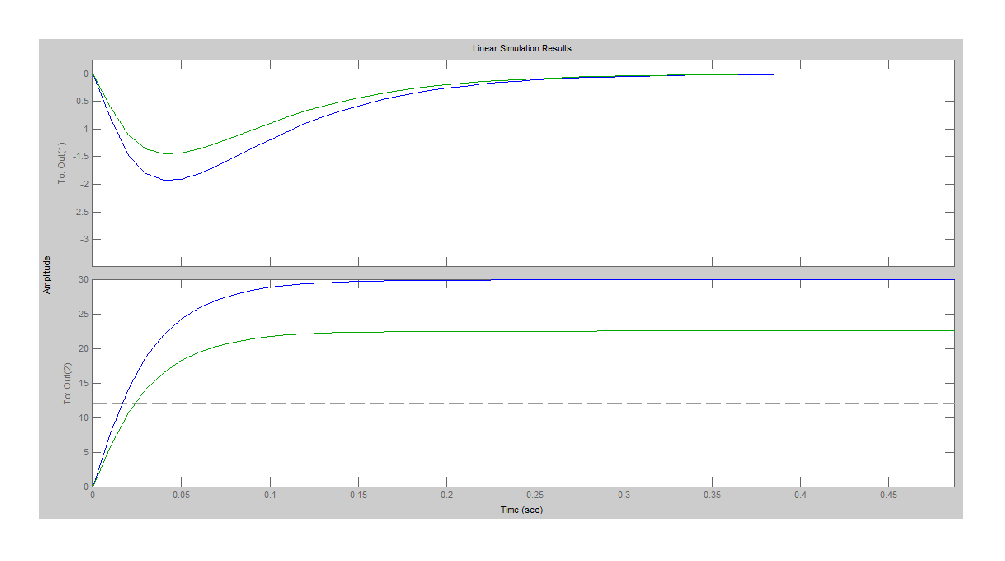
\includegraphics[width=\textwidth,trim=0 0 0 0]{graphics/ZoomOpenLoop.pdf} %trim=l b r t (can cut off from every side)
	\caption{This figure a comparison between the actual model made and the adjusted model.}
	\label{fig:zoom_step}			% figure labels are of the form \label{fig:*}
\end{figure}
On figure \ref{fig:zoom_step} it is seen that the coupling between pan and tilt is insignificant, this means that the system can be decoupled such that the pan does not affect the tilt and visa versa, forming two simple transfer functions as shown in \ref{eq:model_model} the following way:
\begin{align}
	U(s) &= \frac{L J_L}{K_T} s^2 \Omega(s) + \frac{R J_L}{K_T} s \Omega(s) + K_B \Omega(s) \Rightarrow\\
	H(s) &= \frac{\Omega(s)}{U(s)} = \frac{1}{\frac{L J_L}{K_T} s^2 + \frac{R J_L}{K_T} s + K_B}\label{eq:transfer_function}
\end{align}
If parameters for pan and tilt are inserted into equation \ref{eq:transfer_function} the following is obtained:
\begin{align}
	G_{Pan}(s) &= \frac{1}{30.49 \cdot 10^{-6} s^2 + 24.14 \cdot 10^{-3} s + 0.4011}\label{eq:transfer_function_pan}\\
	G_{Tilt}(s) &= \frac{1}{15.65 \cdot 10^{-6} s^2 + 12.39 \cdot 10^{-3} s + 0.4011}\label{eq:transfer_function_tilt}
\end{align}

\section{Discussion}
From models developed throughout this chapter and analysis made on measurements of the actual system, it has been proved that using a state-space model for the pan-tilt system is unnecessary. Therefore two transfer functions have been derived for further analysis of the control system. Decoupling the system was done due to the almost non-existent mutual effect expressed in figure \ref{fig:zoom_step}.

The only still expected gain from using state-space is the possibility of regulating the velocity of the system. This however would only contribute to the settling time of the system and not the precision and is therefore irrelevant according to the purpose of this project.

\subsection{Conclution}
The perspective in developing a state space model was to use it for a full state feedback regulator, but due to the low coupling between the pan and the tilt, this plan is abandoned. This decision has some influence on the other parts of the system, since the need for estimating the velocity is no longer present. Furthermore a classic PID regulator must be developed for each subsystem.